\FloatBarrier

\begin{figure}[h!]
	\centering
	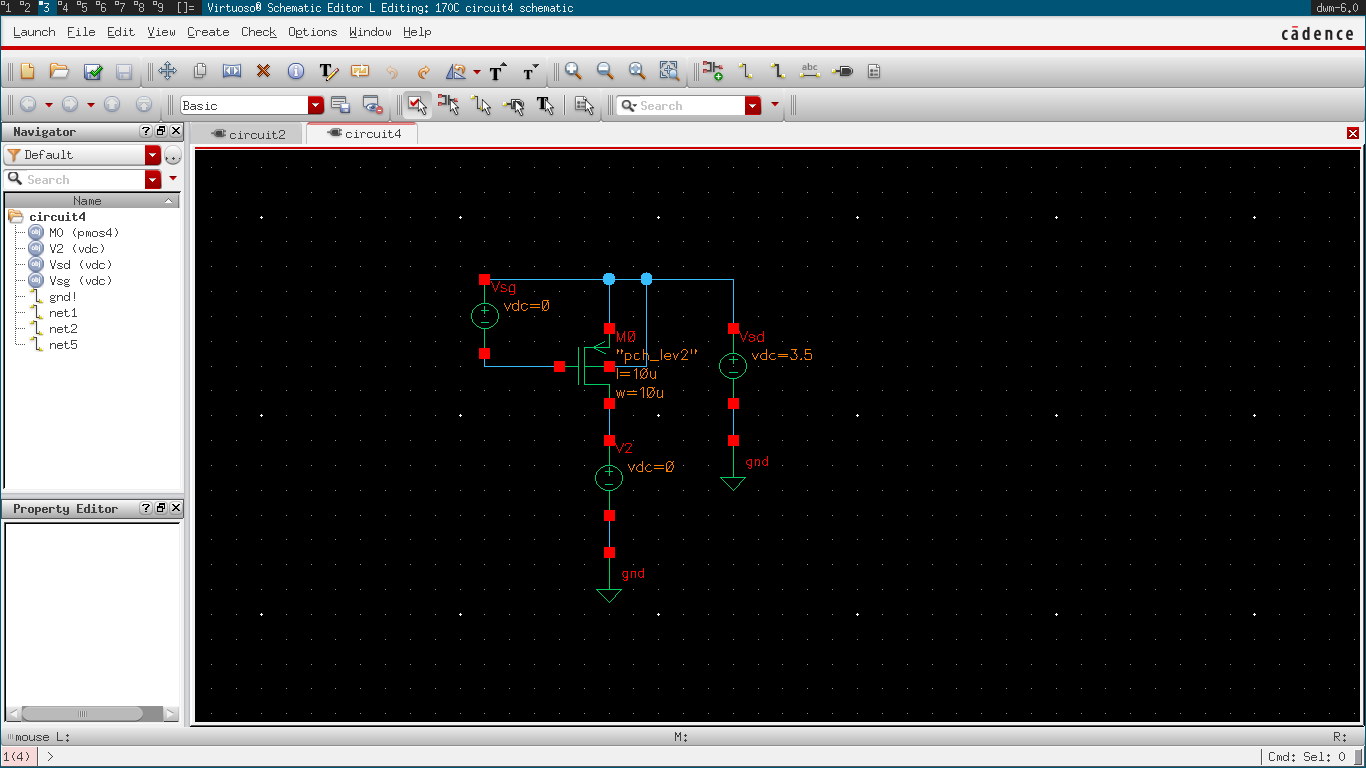
\includegraphics[scale=0.30]{./images/circuit4.PNG}
	\caption{Circuit for Simulation 4}
	\label{fig:circuit4}
\end{figure}

\FloatBarrier
The results for Simulation 4 are similar to Simulation 2, except a PMOS is used instead of an NMOS.
The definition $g_{sd} = \frac{\partial I_{D}}{\partial V_{SD}}$ is used instead.

\FloatBarrier

\begin{figure}[h!]
	\centering
	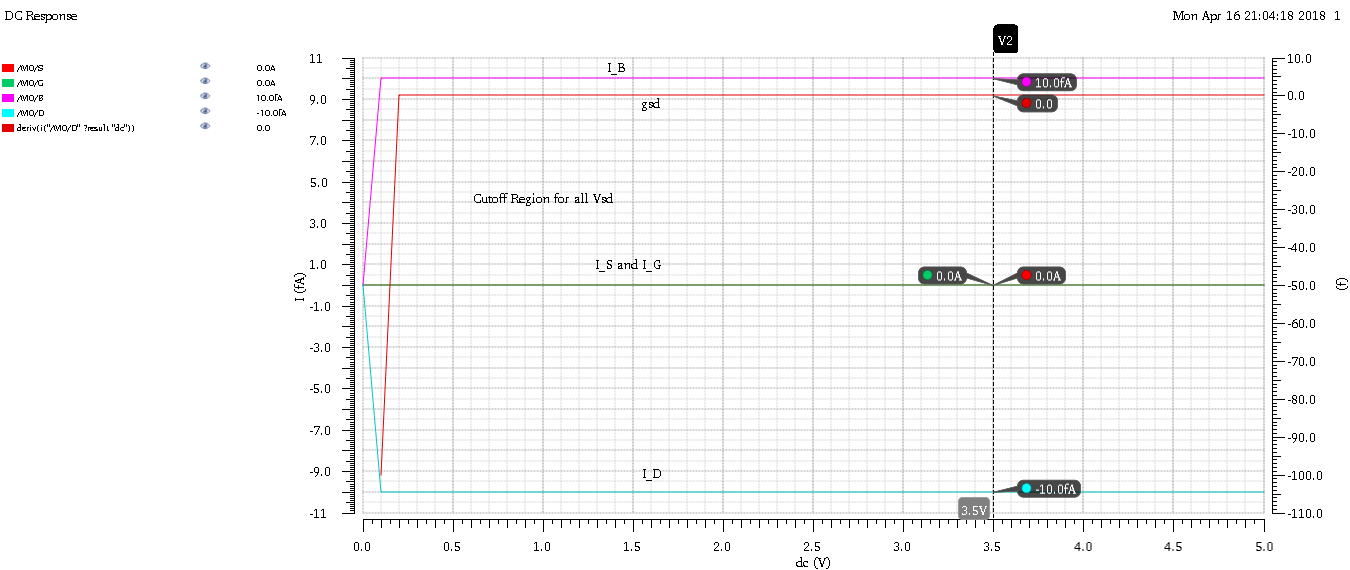
\includegraphics[scale=0.45]{./images/id_vs_vds_vgs_is_0_pmos.PNG}
	\caption{PMOS $I_{D}$ versus $V_{SD}$ when $V_{SG} = 0$\si{\volt}}
	\label{fig:id_vs_vds_vgs_is_0_pmos}
\end{figure}

\FloatBarrier

\FloatBarrier

\begin{figure}[h!]
	\centering
	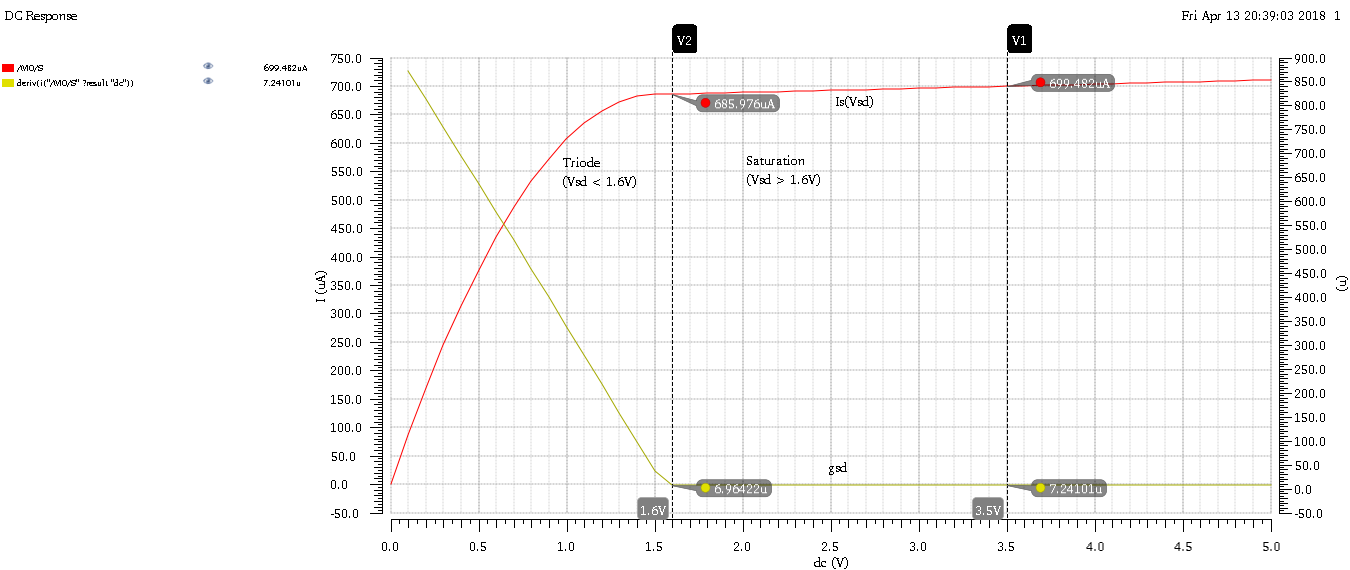
\includegraphics[scale=0.45]{./images/id_vs_vds_vgs_is_2_5_pmos.PNG}
	\caption{PMOS $I_{D}$ versus $V_{SD}$ when $V_{SG} = 2.5$\si{\volt}}
	\label{fig:id_vs_vds_vgs_is_2_5_pmos}
\end{figure}

\FloatBarrier

\FloatBarrier

\begin{figure}[h!]
	\centering
	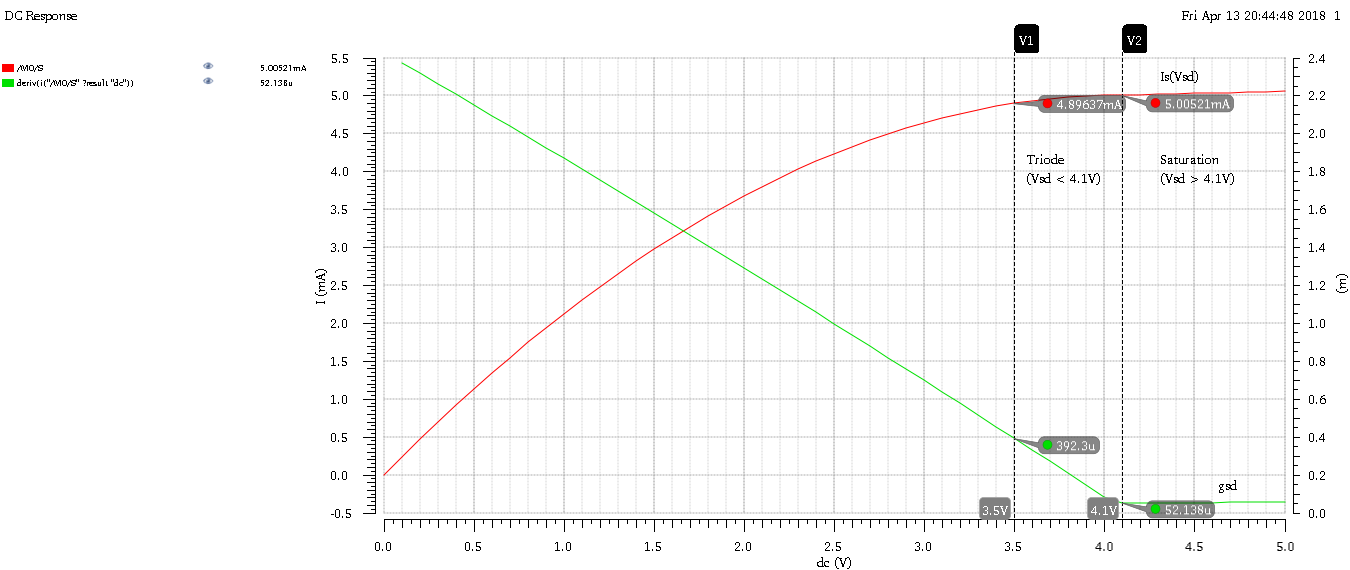
\includegraphics[scale=0.45]{./images/id_vs_vds_vgs_is_5_pmos.PNG}
	\caption{PMOS $I_{D}$ versus $V_{SD}$ when $V_{SG} = 5.0$\si{\volt}}
	\label{fig:id_vs_vds_vgs_is_5_pmos}
\end{figure}

\FloatBarrier

\FloatBarrier

\begin{table}[h!]
	\centering
	\caption{Simulation 4 Results}
	\label{tab:sim4_results}
	\csvautotabular{./tables/sim4_results}
\end{table}

\FloatBarrier

$\lambda$ for the NMOS and PMOS can be calculated from the given data.
Two samples are already taken for each transistor: the current at the edge of saturation and triode $I_{D1}$ and the current at $V_{DS} = 3.5$\si{\volt} (or $V_{SD}$ in the case of a PMOS).
Consider the transistor at $V_{GS} = 2.5$\si{\volt} (or $V_{SG}$ in the case of a PMOS).
It operates in saturation at this $V_{DS}$ (or $V_{SD}$ value).
Therefore, its current is given by $I_{D} = I_{D}' ( 1 + \lambda V_{DS} )$ (or $V_{SD}$ in the case of a PMOS).
So, $\lambda$ can be determined from a system of equations.
The equations are written for the NMOS, but extrapolating to the PMOS is trivial by simply replacing $V_{DS}$ with $V_{SD}$:

\begin{equation}
	\label{eq:lambda_eqn_1}
	I_{D1} = I_{D}' ( 1 + \lambda V_{DS1} )
\end{equation}

\begin{equation}
	\label{eq:lambda_eqn_2}
	I_{D2} = I_{D}' ( 1 + \lambda V_{DS2} )
\end{equation}

Solving equations (\ref{eq:lambda_eqn_1}) and (\ref{eq:lambda_eqn_2}) for $\lambda$ yields:

\begin{equation}
	\label{eq:lambda_solved}
	\lambda = \frac{ I_{D2} - I_{D1} }{ I_{D1} V_{DS2} - I_{D2} V_{DS1} }
\end{equation}

$\lambda$ for each transistor is presented in table(\ref{tab:lambda}).
The results are compared with the simulation models.

\FloatBarrier

\begin{table}[h!]
	\centering
	\caption{Lambda Calculations for Transistors}
	\label{tab:lambda}
	\csvautotabular{./tables/lambda.csv}
\end{table}

\FloatBarrier

A simpler approach can also be taken to determine $\lambda$.
For processes with relatively long transistors, $\lambda$ should not be very large.
Because $\lambda = \frac{1}{V_{A}}$, where $V_{A}$ is the Early voltage, this implies that $V_{A}$ is quite large.
So, long as $V_{DS}$ (or $V_{SD}$ in the case of a PMOS) is not very large relative to $V_{A}$ ($V_{DS} << V_{A}$), the following approximation can be made:

\begin{equation}
	\label{eq:approx_lambda}
	I_{D} = I_{D}' ( 1 + \lambda V_{DS} ) \\
	= I_{D}' ( 1 + \frac{V_{DS}}{V_{A}} ) \\
	\approx I_{D}'
\end{equation}

Therefore, $g_{ds} = \lambda I_{D}' \approx \lambda I_{D}$ for $V_{A} >> V_{DS}$ (or $V_{A} >> V_{SD}$ for a PMOS).
So, $\lambda$ can also be approximated using $\lambda \approx \frac{g_{ds}}{I_{D}}$ (or $g_{sd}$ in the case of a PMOS) provided that these assumptions about the transistor hold.
